\documentclass[11pt,landscape,a4paper,fleqn]{article}
\usepackage[utf8]{inputenc}
\usepackage[ngerman]{babel}
\usepackage{tikz}
\usetikzlibrary{shapes,positioning,arrows,fit,calc,graphs,graphs.standard}
\usepackage[nosf]{kpfonts}
\usepackage[t1]{sourcesanspro}
%\usepackage[lf]{MyriadPro}
%\usepackage[lf,minionint]{MinionPro}
\usepackage{multicol}
\usepackage{wrapfig}
\usepackage[top=0mm,bottom=3mm,left=1mm,right=1mm]{geometry}
\usepackage[framemethod=tikz]{mdframed}
\usepackage{microtype}
\usepackage{mathtools}
\usepackage{ccicons}
\usepackage{hyperref}
\usepackage[inline]{enumitem}
% \PassOptionsToPackage{dvipsnames}{xcolor}
\usepackage{xcolor}
% \usepackage[dvipsnames]{xcolor}

\let\bar\overline
\def\D{\mathcal{D}}

\definecolor{myblue}{cmyk}{1,.72,0,.38}
\definecolor{myorange}{cmyk}{0,0.5,1,0}

\pgfdeclarelayer{background}
\pgfsetlayers{background,main}

\everymath\expandafter{\the\everymath \color{myblue}}
\everydisplay\expandafter{\the\everydisplay \color{myblue}}

\renewcommand{\baselinestretch}{.8}
\pagestyle{empty}

\global\mdfdefinestyle{header}{%
linecolor=gray,linewidth=1pt,%
leftmargin=0mm,rightmargin=0mm,skipbelow=0mm,skipabove=0mm,
}

\newcommand{\header}{
\begin{mdframed}[style=header]
\footnotesize
\sffamily
Cheat sheet\\
Nicolas Wehrli,~page~\thepage~of~2
\end{mdframed}
}

\newcommand{\middot}{~\textperiodcentered~}
\newlist{rowlist}{enumerate*}{1}
\setlist[rowlist]{label={\textbf{\roman*}\text{: }}, afterlabel={}, itemjoin=\middot}

\newcommand{\E}[0]{\mathbb{E}}
\newcommand{\N}[0]{\mathbb{N}}
\newcommand{\R}[0]{\mathbb{R}}

\newcommand{\sgn}[0]{\text{sgn}}

\newcommand{\argmin}[1]{\underset{#1}{\text{argmin}}}
\newcommand{\argmax}[1]{\underset{#1}{\text{argmax}}}


\makeatletter
\renewcommand{\section}{\@startsection{section}{1}{0mm}%
                                {0pt}%
                                {0.5pt}%x
                                {\color{myorange}\sffamily\small\bfseries}}
\renewcommand{\subsection}{\@startsection{subsection}{1}{0mm}%
                                {0pt}%
                                {0.1pt}%x
                                {\sffamily\bfseries}}


\makeatother
\setlength{\parindent}{0pt}

\newcommand{\red}[1]{\textcolor{red}{#1}}
\newcommand\iid{\stackrel{\mathclap{\normalfont\mbox{\tiny{iid}}}}{=}}

\begin{document}
	
\section*{Disclaimer}

\small
\begin{multicols*}{4}
	
This document is an exam summary that follows the slides of the \textit{Introduction to Machine Learning} lecture  at ETH Zurich. 
The contribution to this is a short summary that includes the most important concepts, formulas and algorithms. 
This summary was created during the spring semester 2018 by Yannik Merkli and adapted in 2024 by Nicolas Wehrli. 
Due to updates to the syllabus content, some material may no longer be relevant for future versions of the 
lecture. This work is published as CC BY-NC-SA.

\begin{center}
	\ccbyncsa
\end{center}

I do not guarantee correctness or completeness, nor is this document endorsed by the lecturers. 
Feel free to point out any erratas. 
For the full \LaTeX \ source code, consider \texttt{\href{https://github.com/nwehrli/ymerkli-eth-summaries}{https://github.com/nwehrli/ymerkli-eth-summaries}}.

\newpage
	
%\section*{Probabilities}
$P(X,Y)=P(X|Y)P(Y)=P(Y|X)P(X)\\
P(X,Y|Z)=P(X|Y,Z)P(Y|Z)\\
P(X,Y|Z)=P(Y|X,Z)P(X|Z)$\\
$\text{X,Y iid:}P(X,Y|Z)=P(X|Z)P(Y|Z)$\\
$P(X=x)=\sum_{y'\in Y}P(X=x,Y=y')$\\
$\text{iid:}P(X_1,...,X_n|Y)=\prod_{i=1}^{n}P(X_i|Y)$\\
$\mathbb{E}_x[X] = \begin{cases}
   \int x \cdot p(x) \partial x  &|\mathbb{E}_x[f(x)] =\\
   \sum_x x \cdot p(x) &|\int f(x) \cdot p(x) \partial x
  \end{cases}$\\
%$\mathbb{E}_x[f(x)] = \int f(x) \cdot p(x) \partial x $\\
$\mathbb{E}[X+Y]=\mathbb{E}[X]+\mathbb{E}[Y]$\\
$\sigma_X^2=Var[X] = \mathbb{E}[(X-\mu_X)^2] = \mathbb{E}[X^2] - \mathbb{E}[X]^2$\\
$p(Z|X,\theta) = \frac{p(X,Z|\theta)}{p(X|\theta)}$\\
%\subsection*{Linearity of expectation}
%$X, Y$ rand. var., $a, b \in \mathbb{R}$:\\
%$\mathbb{E}_{x,y}[aX + bY] = a\mathbb{E}_x[X] + b \mathbb{E}_y[Y]$
\section*{Basics}
%-------------------------------------------------------------------------------------------
%PROBABILITIES
%-------------------------------------------------------------------------------------------
% $P(X,Y)=P(X|Y)P(Y)=P(Y|X)P(X)\\
% P(X,Y|Z)=P(X|Y,Z)P(Y|Z)\\
% P(X,Y|Z)=P(Y|X,Z)P(X|Z)$\\
% $P(X,Y,Z)=P(X|Y,Z)P(Y|Z)P(Z)$\\
% $\text{X,Y iid:}P(X,Y|Z)=P(X|Z)P(Y|Z)$\\
% $P(X=x)=\sum_{y'\in Y}P(X=x,Y=y')$\\
% $\text{iid:}P(X_1,...,X_n|Y)=\prod_{i=1}^{n}P(X_i|Y)$\\
% $\mathbb{E}_x[X] = \begin{cases}
% \int x \cdot p(x) \partial x  &|\mathbb{E}_x[f(x)] =\\
% \sum_x x \cdot p(x) &|\int f(x) \cdot p(x) \partial x
% \end{cases}$\\
% %$\mathbb{E}_x[f(x)] = \int f(x) \cdot p(x) \partial x $\\
% $\mathbb{E}[X+Y]=\mathbb{E}[X]+\mathbb{E}[Y]$\\
% $\sigma_X^2=Var[X] = \mathbb{E}[(X-\mu_X)^2] = \mathbb{E}[X^2] - \mathbb{E}[X]^2$\\
% $p(Z|X,\theta) = \frac{p(X,Z|\theta)}{p(X|\theta)}$
%\subsection*{Linearity of expectation}
%$X, Y$ rand. var., $a, b \in \mathbb{R}$:\\
%$\mathbb{E}_{x,y}[aX + bY] = a\mathbb{E}_x[X] + b \mathbb{E}_y[Y]$

%-------------------------------------------------------------------------------------------
%Calculus and stuff
%-------------------------------------------------------------------------------------------


% $ln(x) \leq x - 1, x>0$; $||x||_2 = \sqrt{x^T x}$; $\nabla_x ||x||_2^2 = 2 x$%; $||x||_p = (\sum_{i=1}^n|x_i|^p)^{\frac{1}{p}}$, $1 \leq p < \infty$

% $f(x) = x^T A x$; $\nabla_x f(x) = (A + A^T) x$

% $D_{KL} = \mathbb{E}_p[log(\frac{p(x)}{q(x)})]$; $D_{KL} (P||Q) = \sum_{x \in X}P(x) \cdot log \frac{P(x)}{Q(x)} =  \int_{-\infty}^{+\infty} p(x) log \frac{p(x)}{q(x)} \, dx $ always nonneg

\textbf{Orth:} A: $det(A)\in\{+1,-1\},AA^T=A^TA=I$\\
\(trace(ABC) = trace(BCA) = trace(CAB)\)\\ 
\(trace(A)=\sum \lambda_i(A);
% $, A\in\mathbb{R}^{n\times n}, (A^{-1})^T=(A^T)^{-1}$\\
% $rank(A)=n, det(A)\neq0$\\
\begin{bmatrix}
a&b \\ 
c&d
\end{bmatrix}^{-1}=\frac{1}{ad-bc}
\begin{bmatrix}
d&-b \\ 
-c&a
\end{bmatrix}
\)

\(A=\sum_{k=1}^{rk(A)}\sigma_{k,k}u_k (v_k)^T, A^\dag = U S' V^T; \sigma'_{k, k} = \frac{1}{\sigma_{k,k}}\)

\textbf{Deriv:}
$\frac{\partial}{\partial x}b^Tx=\frac{\partial}{\partial x}x^Tb=b^T,\!
\frac{\partial}{\partial x}||x||_2^2=2x^T,\! \frac{\partial}{\partial x} ||x -a||_2 = \frac{(x-a)^T}{||x-a||_2},\!
\frac{\partial}{\partial x}(x^TAx)=x^T(A^T+A),$
$\frac{\partial}{\partial x}(b^TAx)=A^Tb, \nabla_X(c^TXb)=cb^T,
\nabla_X(c^TX^Tb)=bc^T; ||A||_{op} = sup_{||x||_2=1}||Ax||_2$

$\textbf{convex} \iff f(\lambda x+ (1-\lambda)y) \leq \lambda f(x) + (1-\lambda)f(y); 
f(y) \geq f(x) + \langle\nabla f(x), y-x\rangle; D^2f(x) \geq 0$\\
\(\alpha f + \beta g \textbf{ c.}; \max(f, g) \textbf{ c.} \text{ if } f, g \textbf{ c.}, \alpha, \beta \geq 0\)\\
\(f \circ g = f(g(x)) \textbf{ c.} \text{ if } f \textbf{ c.}, g \textbf{ a.} \lor f \textbf{c., non-dec.}, g \textbf{ c.}\)
% \textbf{Eigdec:}
% $A,Q \in \mathbb{R}^{n\times n}, A=Q\Lambda Q^{-1},\! \Lambda = diag(\lambda_i)$\\
% $Q=[v_1,..,v_n], \text{(col's are e-vec.)}$\\
% $\text{if all $\lambda_i\geq0:$} A^{-1}=Q\Lambda^{-1}Q^{-1},\Lambda^{-1}=diag(\frac{1}{\lambda_i})$\\
% $\text{if }A=A^T\text{(symm.) and }x^TAx\geq0 \forall x \neq 0 \rightarrow psd$\\

% $X\in \mathbb{R}^{n\times p}, U\in \mathbb{R}^{n\times n}, S\in \mathbb{R}^{n\times p},
% V\in \mathbb{R}^{p\times p}$\\
% $X^TX=VS^TU^TUSV^T=VS^TSV^T=V\Sigma V^T$\\
% $\Sigma = diag(\sigma_1^2,..,\sigma_n^2);\sigma_i^2=\lambda_i; \forall \lambda_i \geq 0$
\(p_{\mu, \Sigma}(x)=\frac{1}{\sqrt{(2\pi)^p det(\Sigma)}}\exp(-\frac{1}{2}(x-\mu)^T\Sigma^{-1}(x-\mu))\)\\
\(\mathbf{X} \sim \mathcal{N}(\mu, \Sigma) \implies A\mathbf{X} + b \sim \mathcal{N}(A\mu+b, A\Sigma A^T)\)

% \textbf{Gauss CDF:}\\
% $\Phi(u;v,w) = \int_{-\infty}^{u} \mathcal{N}(y;v,w)dy=\Phi(\frac{u-v}{\sqrt{w}};0,1)$;\\ %CDF: cumulative distribution function; PDF: standard normal probability density function, $\mu = 0$, $\sigma = 1$
%PDF: $\phi(x) = \frac{1}{\sqrt{2\pi}} e^{-(1/2)x^2}$; $\int \phi(x) \partial x = \Phi(x) + c$;\\
%$\int x \phi(x) = -\phi(x) + c$; $\int x^2 \phi(x) \partial x = \Phi(x) -x \phi(x) + c$
\textbf{Jensen ineq: }$g(E[X]) \leq E[g(X)]$, $g$ convex


\section*{Regression}
\subsection*{Linear Regression $f(x)=w^Tx; X \in \mathbb{R}^{n \times d}$}
$L(w) = ||Xw-y||^2_2; X^TX \hat{w} = X^T y$\\
% $\hat{w} = \operatorname{argmin_w} \sum_{i=1}^n (y_i - w^Tx_i)^2$\\
\(d \leq n: \hat{w} = (X^TX)^{-1}X^Ty\) if \(rk(X) = d\)\\
\(n < d: \hat{w} = (X^TX)^\dag X^T y\); \(rk(X) = n\) \(||\hat{w}||_2\) min.

$\nabla_w L(w)  = 2X^T (Xw-y)$
% = -2 \sum_{i=1}^n (y_i-w^T x_i) \cdot x_i
\subsection*{Gradient Descent}
1. Start arbitrary $w_o \in \mathbb{R}$\\
2. Do $w_{t+1} = w_t - \eta \nabla L(w_t)$ until \(||w^t - w^{t-1}||_2 \leq \epsilon\)

GD conv. to \(\hat{w}\) if \(rk(X^TX) = d, \eta < \frac{2}{\lambda_{max}(X^TX)}\)
\(||w^{t+1} - \hat{w}||\leq ||I - \eta X^TX||_{op}||w^t-\hat{w}||_2 \leq 
\rho^{t+1}||w^0-\hat{w}||_2; \eta_{opt} = \frac{2}{\lambda_{max}+\lambda_{min}}; 
\rho_{min} = 1-\eta_{opt}\lambda_{min} = \frac{\kappa-1}{\kappa+1}\)
\textbf{minibatch SGD:} \(\nabla L_S(w)\) on random \(S \subset D\) every iter.; \(|S| = 1\) SGD; 
\(E_S(\nabla L_S(w)) = \nabla L(w)\)

\textbf{strictly c.} \(\implies\) stationary point is unique g. min.;
\textbf{strongly c.} \(\implies\) unique g. min. exists 
\subsection*{Errors}
exp. estim. err.: \(E_X(\ell(f(X), f^*(X)))\); \(y = f^*(x)+\varepsilon\)\\
generaliz. err.: \(L(f; \mathbb{P}_{X,Y}) = E_{X,Y}(\ell(f(X), Y))\)
\(L(\hat{f}; \mathbb{P}_{X,Y}) = E_X((\hat{f}(X) - f^*(X))^2) + \sigma^2\)(sq. loss)
\(L(\hat{f}_\D; \D_{\text{test}}) = 
\frac{1}{|\D_{\text{test}}|}\sum_{(x,y) \in \D_{\text{test}}}
\ell(\hat{f}_\D(x),y)\) estim. generaliz. err.; g. err. + const = exp. estim err.
\textbf{k-fold CV:} \(\uparrow\)k \(\implies\) \(\hat{f}_{M_i, \D'} \approx \hat{f}_{M_i, \mathcal{D_{\text{use}}}}\), 
\(CV_k(M_i) \not \approx L(\hat{f}_{M_i, \D_\text{use}};\mathbb{P}_{X, Y})\); extreme: LOOCV
\subsection*{Bias-Variance Tradeoff}
\(\text{Bias}_{\D}^2(\hat{f}_\D, x) := (E_\D(\hat{f}_\D(x))-f^*(x))^2\)\\
\(\text{Bias}^2_{\D}(\hat{f}_\D) := E_X(\text{Bias}_{\D}^2(\hat{f}_\D, X));
\text{Var}_\D(\hat{f}_\D) := E_X(\text{Var}_\D(\hat{f}_\D(X)));\text{ Pred. err. } 
E_\D(L(\hat{f}_\D; \mathbb{P}_{X,Y})) = \text{Var}_\D(\hat{f}_\D)+\text{Bias}_\D^2(\hat{f}_\D)+\sigma^2\)
% \subsection*{Gaussian/Normal Distribution}
% $\sigma =$ standard deviation, $\sigma^2 =$ var., $\mu =$ mean:\\
% $f(x) = \frac{1}{\sqrt{2\pi\sigma^2}} exp(-\frac{(x-\mu)^2}{2\sigma^2})$\\
% $f(x_1,.,x_k)=\frac{1}{\sqrt{(2\pi)^k|\Sigma|}}
% exp(-\frac{1}{2}(\boldsymbol{x-\mu})^T\Sigma^{-1}(\boldsymbol{x-\mu}))$

\textbf{Ridge} closed form: $\hat{w}=(X^T X + \lambda I)^{-1} X^T y$
\textbf{Kernelized: } \(\min_w \frac{1}{n}||y-\Phi w||_2^2+ \lambda||w||_2^2 = 
\min_{\alpha}\frac{1}{n}||y-K\alpha||_2^2+\lambda\alpha^TK\alpha\)

%\subsection*{L1-regularized regression (the Lasso)}
%Regularization: $\underset{w}{\operatorname{min}} \sum \limits_{i=1}^n (y_i - w^Tx_i)^2 + \lambda ||w||_1$\\
%Encourages coefficients to be exactly 0.

% \subsection*{Standardization}
% Goal: each feature: $\mu = 0$, unit $\sigma^2$: $\tilde{x}_{i,j} = \frac{(x_{i,j}-\hat{\mu}_j)}{\hat{\sigma}_j}$\\
% $\hat{\mu}_j = \frac{1}{n}\sum_{i=1}^n x_{i,j}$, $\hat{\sigma}_j^2 = \frac{1}{n}\sum_{i=1}^n {(x_{i,j}-\hat{\mu}_j)}^2$ 




%\subsection*{Regularization}
%The error term $L$ and the regularization $C$ with regularization parameter $\lambda$: $\min \limits_w L(w) + \lambda C(w)$\\
%L1-regularization for number of features \\
%L2-regularization for the length of $w$

%my idea
%\subsection*{Regularization}
%A lot of supervised learning problems can be written in this way: $\lambda$: $\min \limits_w L(w) + \lambda C(w)$\\
\section*{Classification}
$\hat{y}=sign(f(x))=sign(w^Tx), z = yf(x)$
Surrogate Losses for 0-1: \(\ell_{\text{exp}(z)} = e^{-z}, \ell_{\text{log}}(z) = \log(1+e^{-z})\)

\(\nabla_z \ell_{\text{exp}}\) explodes for \(z \to -\infty\), sens. to outliers.
\textbf{Logistic Reg.} \(L(w) = \frac{1}{n}\sum_{i = 1}^n \log(1+e^{-y_iw^Tx_i})\)
(linear boundary!)


% Perceptron\\
% $l_{P} (w;y_i,x_i) = max\{0, -y_i w^T x_i \}$\\
% $w^* = \operatorname{argmin_w} \sum_{i=1}^n l_p (w;y_i,x_i)$\\
% $\nabla_w l_p(w;y_i,x_i) = (-y_ix_i)1[y_iw^Tx_i<0]$

% \subsection*{Stochastic Gradient Descent (SGD)}
% 1. Start at an arbitrary $w_0 \in \mathbb{R}^d$\\
% 2. For $t = 1, 2,  ...$ do: \\
% 	Pick data point $(x',y') \in_{u.a.r.} D$\\
% 	$w_{t+1} = w_t - \eta_t \nabla_w l(w_t;x',y')$\\
% Perceptron Alg: SGD with Perceptron loss

%\subsection*{Perceptron Algorithm}
%Stoch. Gradient Descent with Perceptron loss\\
%\emph{Theorem:} If $D$ is linearly separable $\Rightarrow$ Perceptron will obtain a linear separator.

%\subsection*{Hinge loss}
%Loss for Support Vector Machine.\\
%$l_H(w;x,y) = max \{0,1-y w^T x\}$

\subsection*{MM and SVM}
\(w_{\text{MM}} = {\arg \max}_{||w||_2=1}\min_{1\leq i \leq n} y_i \langle w, x_i \rangle\)\\
\(w_{\text{SVM}} = \arg \min||w||_2 \text{ s.t. } y_i\langle w, x_i \rangle \geq 1, \forall i\)

If data \textbf{linearly sep.}, 1. \(w_{\text{SVM}} = w_{\text{MM}}||w_{\text{SVM}}||_2\)

2. GD on logistic reg. (\(\eta = 1\)): \(\frac{w^t}{||w^t||_2} \to w_{\text{MM}}\) 

If \textbf{not} and \(ker(X) = \emptyset\), GD on logistic reg. (\(\eta = \frac{4}{\lambda_{max}(X)}\))
\(w^t \to \hat{w}\), \(\hat{w}\) global min.

\textbf{Hinge loss}: $l_H(w;x,y) = max \{0,1-y w^T x\}$\\
\textbf{soft-mar.}
$w^* = \underset{w}{\operatorname{argmin}} ||w||_2^2 + \lambda\sum_{i=1}^nl_H(w;x_i,y_i)\\
g_i(w) = max \{0,1-y_i w^T x_i\} + \lambda ||w||_2^2\\
\nabla_w g_i(w) = \begin{cases}
    -y_i x_i + 2\lambda w &\text{ , if $y_i w^T x_i<1$}\\
		2\lambda w &\text{ , if $y_i w^T x_i \geq 1$}
\end{cases}$

%\subsection*{L1-SVM}
%$\underset{w}{\operatorname{min}} \lambda ||w||_1 + \sum_{i=1}^n max(0,1-y_i w^T x_i)$

%\subsection*{Matrix-Vector Gradient}
%multiply transposed matrix to the same side as its occurance w.r.t. derivate variable: $\beta \in \mathbb{R}^d$
%$\nabla_\beta ( ||y-X\beta||_2^2 + \lambda ||\beta||_2^2 ) = 2X^T (y-X\beta) + 2\lambda \beta$\\

\subsection*{Multi-Class Classification}
\(\hat{y}(x)=\operatorname{argmax_{k \in \{1,.,K\}}}f_k(x)\); \(f = (f_1, ..., f_K)\)\\
\textbf{OvR}: For each class \(k \in [K]\):

1. Relabel \(\tilde{y}_i = 1\) if \(y_i = k\), else \(\tilde{y}_i = -1\) as \(\D_k\)

2. Train \(f_k\) as binary classifier on \(\D_k\) 

\textbf{Cross-E. Loss}: \(\ell_{\text{ce}}(f(x), y) = -\log\left(\frac{e^{f_y(x)}}{\sum_{k=1}^Ke^{f_k(x)}}\right)\)

\textbf{OvO}: \(L(w) = \sum_{i = 1}^n\ell_{\text{ce}}(f_w(x_i), y_i)\); GD on \(L(w)\)

Multiplicative noise model: \(y = y^*(x)\varepsilon\)
\subsection*{Cost Sensitive Classification}
Replace loss by: $l_{CS}(w;x,y) = c_y l(w;x,y)$

\subsection*{Metrics (convention: positive = rare)}
Accuracy=$\frac{\text{\#correct predictions}}{\#all\, predictions}$=$\frac{TP+TN}{TP+TN+FP+FN}$, 
Precision=$\frac{\#correct'+'predictions}{\#all'+'predictions}$=$\frac{TP}{TP+FP}=$1-FDR\\
Rec.=TPR=$\frac{TP}{TP+FN}=\frac{TP}{n_+}$, FPR=$\frac{FP}{TN+FP}=\frac{FP}{n_-}$=T1\\
F1 score $=\frac{2TP}{2TP+FP+FN}=\frac{2}{\frac{1}{Precision}+\frac{1}{Recall}}$

\(\hat{y_\tau}(x) = \text{sign}(\hat{f}(x) - \tau)\) (varying threshold)
\section*{Kernels $k: \mathcal{X} \times \mathcal{X} \rightarrow \mathbb{R}$}

Reparam. \(w = \phi^T\alpha\); \(f(x) = \sum_{i=1}^n\alpha_i\langle\phi(x_i), \phi(x)\rangle\)

A kernel is \textbf{valid} if $K$ is sym.: $k(x,z) = k(z,x)$ and psd: $z^\top K z \geq 0$

\textbf{mono.}: $k(x,y) = (x^\top y)^m$,
\textbf{poly}: $k(x,y) = (1+x^\top y)^m$,
\textbf{RBF}: $k(x, z) = \exp ( -\frac{||x - z||_\alpha}{\tau} )$, $\alpha = 1 \Rightarrow $ Laplacian, $\alpha = 2 \Rightarrow $ Gaussian

\textbf{Mercers Theorem}: Valid kernels can be decomposed into a lin. comb. of inner products.

\textbf{Kernel composition}
$k = k_1 + k_2$, 
$k = k_1 \cdot k_2$,
$\forall c > 0. \; k = c \cdot k_1$,
$k = f(k_1)$, $f$ pwr. series w/ non-neg. coeffs.,
$k(\binom{x}{y}, \binom{x'}{y'})=k(x,x')k(y,y')$, $k(\binom{x}{y}, \binom{x'}{y'})=k(x,x') + k(y,y')$,
$k(x, x') = g(\left< x, x' \right>)$, $g$ all Taylor coefficients non-negative,
$\forall f. \; k(x,y) = f(x)k_1(x,y)f(y)$

\textbf{Kern. Ridge Reg.}
$\min_w \frac1n \|y - \Phi w\|^2 + \lambda ||w||_2^2 = \min_\alpha \frac1n ||y - K\alpha||_2^2 + \lambda \alpha^\top K \alpha$


\subsection*{k Nearest Neighbor classifier}
% $y=sign(\sum_{i=1}^n y_i [x_i \text{ among k nn of } x])$
\begin{rowlist}
	\item Pick $k$ and distance metric $d$
	\item For given $x$, find among $x_1,...,x_n \in D$ the $k$ closest to $x \to x_{i_1},..., x_{i_k}$
	\item Output the majority vote of labels
\end{rowlist}

% \section*{Multi-class Hinge Loss}
$l_{MC-H}(w^{(1)},...,w^{(c)};x,y) =\\
\operatorname{max_{j \in \{[1,..,c]\setminus y\}}}(0,1+\text{max } w^{(j)T} x - w^{(y)T} x)$
\section*{Neural Networks}
$F(x)=W^{L}\phi^{L-1}(W^{L-1}...(\phi^{1}(W^{1}x)...))$

$\textbf{ReLU: } \max (0,z), \; \textbf{Tanh: } \frac{\exp(z) - \exp(-z)}{\exp(z) + \exp(-z)}$ \\[-3pt]
$\textbf{Sigmoid: } \varphi(z) = \frac{1}{1 + \exp(-z)}, \varphi' = (1 - \varphi) \varphi$


\textbf{Universal Approximation Theorem}: We can approximate any arbitrary smooth target function, with 1+ layer with sufficient width.

\subsection*{Forward Propagation}

Input: $v^{(0)} = [x; 1]$ \quad Output: $f = W^{(L)} v^{(L-1)}$
Hidden: $z^{(l)} = W^{(l)} v^{(l-1)}, v^{(l)} = [\varphi(z^{(l)}); 1]$

\subsection*{Backpropagation}

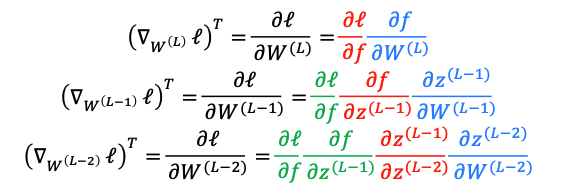
\includegraphics[width=\columnwidth]{assets/backpropagation.png} \\[-15pt]



Only compute {\color{red} \textbf{the gradient}}. Rand. init. weights by distr. assumption for $\varphi$. ( $2 / n_{in}$ for ReLu and $1/n_{in}$ or $ 2/ (n_{in} + n_{out})$ for Tanh)

\subsection*{Overfitting}
\textbf{Regularization}; \textbf{Early Stopping}; \textbf{Dropout}: 
ignore hidden units with prob. $1-p$, after training use all units 
and scale weights by $p$; 
\textbf{Batch Normalization}: normalize the input data 
for each mini-batch, rescale and shift;

\subsection*{CNN \quad \color{black}$\varphi(W * v^{(l)})$}

The out. dim. of applying $k$ $f \times f \times d$ filters (\(d\) = \# channels) to 
$n \times m$ image with padding $p$ and stride $s$ is: 
$\left(\frac{n+2p-f}{s}+1\right) \times \left(\frac{m+2p-f}{s}+1\right)$ with \(k\) channels.
If \(t\times t\) pooling is applied, both dimensions are divided by \(t\), nr. channels stays.
\textbf{Don't forget bias}: 1 per filter + \#outputs for any fully connected layer.

\subsection*{Learning with momentum}
$a \leftarrow m \cdot a + \eta_t \nabla_W l(W;y,x)$; $W \leftarrow W - a$
\section*{Clustering}
\subsection*{k-mean}
$\hat{R}(\mu) = \sum_{i=1}^n \underset{j\in\{1,...k\}}{\operatorname{min}}||x_i-\mu_j||_2^2$, 
non-convex, NP-hard, kernelizable, local opt., spherical bias\\
\textbf{Algorithm (Lloyd's heuristic):}\\
Initialize cluster centers $\mu^{(0)} = [\mu_1^{(0)},...,\mu_k^{(0)}]$\\
While still changes in assignments:\\
$z_i^{(t)} = \underset{j\in\{1,...,k\}}{\operatorname{argmin}}||x_i - \mu_j^{(t-1)}||_2^2$; $\mu_j^{(t)} = \frac{1}{n_j^{(t)}}\sum_{i:z_i^{(t)}=j}x_i$\\
\(\mathcal{O}(nkd)\)  per it., worst-case exponential it. 

Conv. proof: \(\hat{R}(\mu, z) := \sum_{i = 1}^n ||x_i - \mu_{z_i}||_2^2\).
\(\hat{R}(\mu^{(t)}, z^{(t)}) \geq \hat{R}(\mu^{(t)}, z^{(t+1)}) \geq \hat{R}(\mu^{(t+1)}, z^{(t+1)})\) 
\subsection*{k-mean++}
- Start with random data point as center\\
- for $j=2$ to $k$:
$i_j$ sampled with prob.\\
$P(i_j=i) = \frac{1}{z} \underset{1\leq l<j}{min}||x_i-\mu_l||_2^2$; $\mu_j \leftarrow x_{i_j}$

in exp. conv. to \(\mathcal{O}(\log k) \cdot \)OPT

Selecting \(k\): elbow method, regularization

\section*{Dimension Reduction}
\subsection*{Principal component analysis (PCA)}
Given: $D=\{x_1,...,x_n\} \subset \mathbb{R}^d$, $1\leq k \leq d$\\
$\Sigma_{d \times d} = \frac{1}{n}\sum_{i=1}^n x_i x_i^T$, $\mu =\frac{1}{n}\sum_{i = 1}^n x_i = 0$ !!\\
Sol.:
$(W,z_1,...,z_n) = \operatorname{argmin} \sum_{i=1}^n||W z_i - x_i||_2^2$,\\
where $W \in \mathbb{R}^{d \times k}: W^TW = I_k$, $W^* = (v_1|...|v_k)$ w/ $v_i$ evec. of $\Sigma$ and evals $\lambda_1 \geq ... \geq \lambda_d \geq 0$.\\
Projections $z_1,...,z_n\in\mathbb{R}^k$ are given by\\
$z_i = W^T x_i$ where $\Sigma = \sum_{i=1}^d \lambda_i v_i v_i^T$, 

\textbf{Kernel PCA}\\
%$\alpha*=\operatorname{argmax_{\alpha^TK\alpha=1}}\alpha^TK^TK\alpha$\\
For general $k\geq1$, the Kernel PC are given by $\alpha^{(1)},...,\alpha^{(k)}\in \mathbb{R}^n$, where $\alpha^{(i)} = \frac{1}{\sqrt{\lambda_i}}v_i$ is obtained from: $K = \sum_{i=1}^n \lambda_i v_i v_i^T$, $\lambda_1 \geq ... \geq \lambda_d \geq 0$\\
Point $x$ projected as $z \in \mathbb{R}^k$:
$z_i = \sum_{j=1}^n\alpha_j^{(i)}k(x,x_j)$

\subsection*{Autoencoders $f_1: \mathbb{R}^d \rightarrow \mathbb{R}^k, f_2:\mathbb{R}^k \rightarrow \mathbb{R}^d$}
Try to learn identity function: $x \approx f(x;\theta)$\\
$f(x;\theta) = f_2(f_1(x_1;\theta_1);\theta_2)$; $f_1:$ en-, $f_2:$ decoder\\
Lin. activation func. \& square loss $=>$ PCA
% $ W^*=\operatorname{argmin_w}\sum_{i=1}^n||x_i-W^{(2)}\varphi(W^{(1)}x^{(i)})||_2^2$\\
% $\varphi(z)=z: NNA=PCA, w^{(1)}=PCA(x)=w^{(2)^T}$
\section*{Probability Modeling}
Assumption: Data set is generated iid\\
Find $h:X\rightarrow Y$ that minimizes pred. error 

$\hat{y} =h^*(x) = \mathbb{E}[Y|X=x]$ for sq. loss

\subsection*{Maximum Likelihood Estimation (MLE)}
Choose a particular parametric $\hat{p}(Y|X,\theta)$

\(\theta^* = \underset{\theta}{\operatorname{amax}} \hat{p}(y_{1:n}|x_{1:n},\theta)\\\iid 
    \operatorname{amin_\theta} - \sum_{i=1}^n log \hat{p}(y_i|x_i,\theta)\)

\subsection*{Ex. Conditional Linear Gaussian}

Assume Gaussian noise $y = f(x) + \epsilon$ with $\epsilon \sim \mathcal{N}(0, \sigma^2)$ and $f(x) = w^\top x$:

\qquad \qquad $\hat p(y \; | \; x, \theta) = \mathcal{N}(y; w^\top x, \sigma^2)$

The optimal $\hat w$ can be found using MLE:

$\hat w = \argmax{w} \; p(y | x, \theta) =\argmin{w} \sum (y_i - w^\top x_i)^2$
\subsection*{Maximum a Posteriori Estimate}

Assume $y = f(x; \theta^*) + \epsilon$, $\epsilon \sim \mathcal{N}(0, \sigma^2)$, but $\theta^* \sim \mathcal{N}(0, \sigma_\theta^2 I_d)$ The posterior distribution of $\theta$ is given by:
$p(\theta \; | \; \mathcal{D}) = \frac{p( \mathcal{D} \; | \; \theta)}{p( \mathcal{D})} \cdot p(\theta)$

Now we want to find the MAP for $\theta$:

$\hat \theta = \text{argmax}_\theta \; p(\theta \; | \; \mathcal{D})$

\quad $= \text{argmax}_\theta \; p(\mathcal{D} \; | \; \theta) \cdot p(\theta)$

\quad $= \text{argmin}_\theta - \sum_{i=1}^n \log p(y_i \; | \; x_i, \theta) - \log p(\theta)$

\quad $= \text{argmin}_\theta \; \frac{\sigma^2}{\sigma_\theta^2} ||\theta||_2^2 + \sum_{i=1}^n(y_i - f(x_i; \theta))^2$

Regularization can be understood as MAP inference, with different priors (= regularizers) and likelihoods (= loss functions).


\subsection*{Statistical Models for Classification}

$f$ minimizing the population risk: $f^*(x) = \text{argmax}_{\hat y} \; p(\hat y \; | \; x)$

This is called the Bayes' optimal predictor for the 0-1 loss. Assuming iid. Bernoulli noise, the conditional probability is:

\qquad \qquad$p(y \; | \; x,w) \sim \text{Ber}(y; \sigma(w^\top x))$

Where $\sigma(z) = \frac{1}{1 + \exp(-z)}$ is the sigmoid function. Using MLE we get:

\quad \;$\hat w = \argmin{w} \sum_{i = 1}^n \log (1 + \exp(-y_i w^\top x_i))$

Which is the logistic loss. Instead of MLE we can estimate MAP, e.g. with a Gaussian prior:

$\; \;\hat w = \argmin{w} \; \lambda ||w||_2^2 + \sum_{i = 1}^n \log (1 + e^{-y_i w^\top x_i})$

% \subsection*{Logistic regression}
% Assume iid Bernoulli noise instead of Gauss.\\
% $P(y|x,w) = Ber(y; \sigma(w^Tx)) = \frac{1}{1+exp(-y w^T x)}$\\
% $l_{logistic}(w;x_i,y_i)=log(1+exp(-y_iw^Tx_i))$\\
% $\nabla_wl(w)=\frac{(-y_ix_i)}{1+exp(+y_iw^Tx_i)}=P(Y=-y|x,w)(-y_ix_i)$
% %$=\begin{cases}
% %1/(1+exp(-w^Tx)) = \sigma(w^T x)\\
% %		1 - 1/(1+exp(-w^Tx)) = \sigma (-w^T x)\\
% %\end{cases}$
% %Learning: $w = \underset{w}{\operatorname{argmax}} P(w|x,y)$\\
% %Classification: Use $P(y|x,w) = \frac{1}{1+exp(-yw^Tx)}$ and predict most likely class label.

% \subsection*{Example: MLE for logistic regression}
% $\operatorname{argmax_w} P(y_{1:n}|w,x_{1:n})\\
% = \operatorname{argmin_w} - \sum_{i=1}^n log P(y_i|w,x_i)\\
% = \operatorname{argmin_w} \sum_{i=1}^n log(1+exp(-y_i w^T x_i))\\
% \hat{R}(w) = \sum_{i=1}^n log(1+exp(-y_i w^T x_i))$ (neg log l. f.)
% %negative log likelihood function

% %\subsection*{Gradient for logistic regression}
% %Loss function $l(w) = log(1+exp(-yw^Tx))$\\
% %$\nabla_w l(w) = \frac{1}{1+exp(-yw^Tx)} exp(-yw^Tx) (-yx)$\\
% %$=\frac{1}{1+exp(yw^Tx)} (-yx)$\\
% %$=P(Y = -y|w, x) (-yx)$

% \subsection*{Logistic regression and regularization}
% $\underset{w}{\operatorname{min}} \sum_{i=1}^n log(1+exp(-y_i w^T x_i)) + 
% \lambda (||w||_1 or ||w||_2^2)$

% \subsection*{SGD for logistic regression}
% \iffalse
% 1. Initialize w\\
% 2. For t=1,2,...\\
% Pick data $(x,y) \in_{u.a.r} D$\\
% Prob. of misclas. $\hat{P}(Y = -y|w,x) = \frac{1}{1+exp(yw^Tx)}$\\
% \fi
% Update $w \leftarrow w + \eta_t y x \hat{P}(Y = -y|w,x)$\\
% \textbf{L2 regularized logistic regression:}\\
% Update $w \leftarrow w (1-2\lambda \eta_t) + \eta_t y x \hat{P}(Y = -y|w,x)$

% \subsection*{Multiclass Logistic Regression}
% $P(Y=i|x,w_1,..,w_c)=exp(w_i^Tx)/\Sigma_j^c exp(w_j^Tx)$

\section*{Bayesian Decision Theory}

Given $p(y \; | \; x)$, a set of actions $A$ and a cost $C: Y \times A \mapsto \R$, pick the action with the maximum expected utility. 

\qquad \qquad $a^* = \text{argmin}_{a \in A} \; \E_y[C(y,a) \; | \; x]$

Can be used for asymmetric costs or abstention.
% \section*{Bayesian decision theory}
% - Conditional distribution over labels $P(y|x)$\\
% - Set of actions $\mathcal{A}$
% - Cost function $C:Y\times \mathcal{A} \rightarrow \mathbb{R}$\\
% Pick action that minimizes the expected cost:
% $a^* = \operatorname{argmin_{a \in \mathcal{A}}} \mathbb{E}_y[C(y,a)|x] = \sum_y P(y|x)C(y,a)$\\
% $\mathbb{E}_y[C(y,+)|x]=P(-|x)C(-,+);$\\
% $\mathbb{E}_y[C(y,-)|x]=P(+|x)C(+,-);$\\
% $\mathbb{E}_y[C(y,D)|x]=P(+|x)C_{d+}+P(-|x)C_{d-}$

% \subsection*{Optimal decision for logistic regression}
% $a^* = \operatorname{argmin_y} \hat{P}(y|x) = sign(w^T x)$

% \subsection*{Example: logistic regression}
% \begin{itemize}
% 	 Est. cond. dist: $P(y|x,w) = Ber(\sigma(w^Tx))$
% 	 Action set: $\mathcal{A} = \{ +1, -1\}$
% 	 Cost function: $C(y,a) = [y \not = a]$ \\ 
% 	$= \left \{ 
% 		\begin{array}{lr}
% 			1 \text{ , if } y \not = a\\
% 			0 \text{ , otherwise}
% 		\end{array}
% 		$
% \end{itemize}
% $a^* = \underset{a \in \mathcal{A}}{\operatorname{argmin}} \mathbb{E}_y[C(y,a)|x]$\\
% $= \underset{a \in \mathcal{A}}{\operatorname{argmin}} P(y=1|x,w)[a=1] + P(Y=-1|x,w)[a=+1]$\\
% $= \underset{a \in \mathcal{A}}{\operatorname{argmin}} P(y \not = a | x,w) = \underset{a \in \mathcal{A}}{\operatorname{argmin}} \frac{1}{1+exp(aw^Tx)}$\\
% $=\underset{a \in \mathcal{A}}{\operatorname{argmax}} (1 + exp(aw^Tx))$
% $=\underset{a \in \mathcal{A}}{\operatorname{argmax}} (aw^Tx)$\\
% $= sign (w^Tx)$

%\subsection*{Example: Asymmetric costs}
%	 Est. cond. dist: $\hat{P}(y|x,w) = Ber(\sigma(w^Tx))$
%	 Action set: $\mathcal{A} = \{ +1, -1\}$
%	 Cost function: $C(y,a) =
%	 \begin{cases}
%	 	c_{FP} \text{ , if $y=-1$ and $y=+1$}\\
%			c_{FN} \text{ , if $y=+1$ and $y=-1$}\\
%			0 \text{ , otherwise}
%	 \end{cases}
%		$
%The action that minimizes the expected cost is:\\
%$C_+ = \mathbb{E}_y[C(y,+1)|x] = P(y=+1|x) \cdot 0 + (P(y=-1)|x) \cdot c_{FP}$\\
%$C_- = \mathbb{E}_y[C(y,-1)|x] = P(y=+1|x) \cdot c_{FN} + P(y=-1|x) \cdot 0$\\
%Predict +1 if $C_+ \leq C_- \Leftrightarrow P(y=+1|x) \geq \frac{c_{FP}}{c_{FP} + c_{FN}}$

% \subsection*{Doubtful logistic regression}
% 	 Est. cond. distr.: $\hat{P}(y|x) = Ber(y;\sigma(\hat{w}^Tx))$\\
% 	 Action set: $\mathcal{A} = \{ +1, -1, D\}$;  Cost function:\\
% 	 $C(y,a) = \begin{cases}
% 			[y \neq a] &\text{if } a \in \{+1,-1\}\\
% 			c &\text{if } a = D
%        \end{cases}$\\
% $\rightarrow a^* = y \text{ if } \hat{P}(y|x) \geq 1-c\text{, D otherwise}$
%$a^* = \begin{cases}
%		y &\hat{P}(y|x) \geq 1-c\\
%		D &\text{otherwise}
%	   \end{cases}
%$

% \subsection*{Linear regression}
% 	 Est. cond. distr.: $\hat{P}(y|x,w) = \mathcal{N}(y;w^Tx, \sigma^2)$\\
%  $\mathcal{A} = \mathbb{R}$; $C(y,a) = (y-a)^2$\\
% $\rightarrow a^* = \mathbb{E}_y[y|x] = \int \hat{P}(y | x) \partial y = \hat{w}^Tx$

% \subsection*{Asymmetric cost for regression}
% 	 Est. cond. distr.: $\hat{P}(y|x) = \mathcal{N}(\hat{y};\hat{w}^Tx, \sigma^2)$\\
% 	 $\mathcal{A} = \mathbb{R}$; $C(y,a) = c_1 \max(y-a,0) + c_2 \max(a-y,0)$
% $\rightarrow a^* = \hat{w}^Tx + \sigma \Phi^{-1} (\frac{c_1}{c_1 + c_2})$, $\Phi$: Gaussian CDF
%$\frac{\partial}{\partial a}$\\
%$\frac{\partial}{\partial a} \mathbb{E}_y[C(y,a)|x] = \int_{-\infty}^{\infty} C(y,a) P(y | x) dy \overset{!}{=} 0$\\
%$= -c_1 \int_{a}^{\infty} P(y | x) dy + c_2 \int_{-\infty}^{a} P(y | x) dy$\\
%$= -c_1 [1-\phi(a; w^Tx, \sigma^2)] + c_2 \phi(a; w^Tx, \sigma^2)$\\
%$\phi(a; w^Tx, \sigma^2) = \frac{c_1}{c_1 + c_2}$\\
%using $\phi(u;v,w) = \phi((u-v)/\sqrt{w};0,1)$ and applying inverse CDF of std. ND $\phi^{-1}$ we get\\
%$a^* = w^Tx + \sigma\phi^{-1} (\frac{c_1}{c_1 + c_2})$
\section*{Generative Modeling}

Aim to estimate $p(x, y)$ for complex situations using Bayes' rule: $p(x,y) = p(x|y) \cdot p(y)$

\subsection*{Gaussian Bayes Classifier}

No independence assumption, model the features with a multivariate Gaussian $\mathcal{N}(x; \mu_y, \Sigma_y)$:

\quad $\mu_{y} = \frac{1}{\text{Count}(Y = y)} \sum_{j \; | \; y_j = y} x_{j}$

\quad $\Sigma_{y} = \frac{1}{\text{Count}(Y = y)} \sum_{j \; | \; y_j = y} (x_{j} - \hat \mu_{y}) (x_{j} - \hat \mu_{y})^\top$

This is also called the \textbf{quadratic discriminant analysis} (QDA). LDA: $\Sigma_+ = \Sigma_-$, Fisher LDA: $p(y) = \frac{1}{2}$, classify $x$ as outlier if: $p(x) \leq \tau$.

\subsection*{Gaussian Naive Bayes Classifier}

GBC with diagonal $\Sigma$s (assume features independent). Estimate the parameters via MLE:

MLE for class prior: $p(y) = \hat p_y = \frac{\text{Count}(Y = y)}{n}$
MLE for feature distribution:

\qquad \qquad $p(x_i \; | \; y) = \mathcal{N}(x_i; \hat \mu_{y,i}, \sigma^2_{y,i})$ \\[-10pt]

Where:\\[-12pt]

\qquad \quad $\mu_{y,i} = \frac{1}{\text{Count}(Y = y)} \sum_{j \; | \; y_j = y} x_{j,i}$

\qquad \quad $\sigma^2_{y,i} = \frac{1}{\text{Count}(Y = y)} \sum_{j \; | \; y_j = y} (x_{j,i} - \hat \mu_{y, i})^2$


Predictions are made by: \\[-20pt]
$$y = \argmax{\hat y} \; p(\hat y \; | \; x) = \argmax{\hat y} \; p(\hat y) \cdot \prod_{i=1}^d p(x_i \; | \; \hat y)$$\\[-10pt]
Equivalent to decision rule for bin. class.: \\[-8pt]

\qquad \qquad $y = \sgn \left( \color{red} \log \frac{p(Y = +1 \; | \; x)}{p(Y = -1 \; | \; x)} \color{black} \right)$ \\[-3pt]

Where \color{red}$f(x)$\color{black} is called the discriminant function. If the conditional independence assumption is violated, the classifier can be overconfident.

\subsection*{Avoiding Overfitting}

MLE is prone to overfitting. Avoid this by restricting model class (fewer parameters, e.g. GNB) or using priors (restrict param. values).

\subsection*{Generative vs. Discriminative}

\textbf{Discriminative models}:

$p(y | x)$, can't detect outliers, more robust

\textbf{Generative models}:

$p(x,y)$, can be more powerful (detect outliers, missing values) if assumptions are met, are typically less robust against outliers


% \section*{Discriminative vs. Generative Modeling}
% Discriminative models: aim to estimate $P(y|x)$\\
% G. m.:  aim to estimate joint distribution $P(y,x)$

% Typical approach to generative modeling:\\
% - Estimate prior on labels $P(y)$\\
% - Estimate cond. distr. $P(x|y)$ for each class y\\
% - Obtain predictive distr. using Bayes' rule:\\
% $P(y|x) = \frac{P(y) P(x|y)}{P(x)} = \frac{P(x,y)}{P(x)}$, $P(x) = \sum_y P(x,y)$

% %\subsection*{Example: Naive Bayes Model}
% %cond. ind.:$P(X_1,...,X_d|Y) = \prod_{i=1}^d P(X_i|Y)$

% \subsection*{Example MLE for P(y)}
% Want: $P(Y=1) = p, P(y=-1) = 1-p$\\
% Given: $D=\{(x_1,y_1),...,(x_n,y_n)\}$\\
% $P(D|p) = \prod_{i=1}^n p^{1[y_i=+1]} (1-p)^{1[y_i=-1]}$\\
% $=p^{n_+} (1-p)^{n_-}$, where $n_+ = $ \# of $y=+1$\\
% $\frac{\partial}{\partial p} log P(D|p) = n_+ \frac{1}{p} - n_- \frac{1}{1-p} \overset{!}{=} 0 \Rightarrow p=\frac{n_+}{n_+ + n_-}$

% \subsection*{Example MLE for P=(x|y)}
% Assume: $P(X=x_i|y) = \mathcal{N}(x_i;\mu_{i,y}, \sigma_{i,y}^2)$\\
% Given: $D, D_{x_i|y} = \{x \text{, s.t. } x_{j,i}=x, y_j=y\}$\\
% Thus MLE yields:
% $\hat{\mu}_{i,y} = \frac{1}{n_y} \sum_{x\in D_{x_i|y}} x$;\\ %,where $n_y=|D_{x_i|y}|$\\
% $\hat{\sigma}_{i,y}^2 = \frac{1}{n_y} \sum_{x\in D_{x_i|y}} (x-\hat{\mu}_{i,y})^2$

% \subsection*{Deriving decision rule}
% %In order to predict label y for new point x, use\\
% $P(y|x) = \frac{1}{Z} P(y)P(x|y)$, $Z = \sum_y P(y) P(x|y)$\\
% $y = \operatorname{argmax_{y'}} P(y'|x) = \operatorname{argmax_{y'}} P(y') \prod_{i=1}^d P(x_i|y')\\
% = \operatorname{argmax_{y'}} log P(y') + \sum_{i=1}^d log P(x_i|y')$

% \subsection*{Gaussian Naive Bayes classifier}
% Indep. feat. giv. Y: $P(X_1,..,X_n|Y) = \Pi_{i=1}^dP(X_i|Y)$\\
% MLE for class prior: $\hat{P}(Y=y) = \hat{p}_y = \frac{\operatorname{Count(Y = y)}}{n}$\\
% MLE for feature distr.: $\hat{P}(x_i|y_i) =  \mathcal{N}(x_i;\hat{\mu}_{y,i}, \sigma_{y,i}^2)$\\
% $\hat{\mu}_{y,i} = \frac{1}{\operatorname{Count}(Y=y)} \sum_{j:y_j=y} x_{j,i}$\\
% $\sigma_{y,i}^2 = \frac{1}{\operatorname{Count}(Y=y)} \sum_{j:y_j=y} (x_{j,i} - \hat{\mu}_{y,i})^2$\\
% Prediction given new point x:\\
% $y = \operatorname{argmax_{y'}} \hat{P}(y'|x) = \operatorname{argmax_{y'}} \hat{P}(y') \prod_{i=1}^d \hat{P}(x_i|y')$

% \subsection*{Categorical Naive Bayes Classifier}
% MLE class prior: $\hat{P}(Y=y) = p_y = \frac{Count(Y=y)}{n}$\\
% MLE for feature distr.:
% $\hat{P}(X_i = c|Y = y) = \theta_{c|y}^{(i)}\\
% \theta_{c|y}^{(i)} = \frac{Count(X_i = c, Y = y)}{Count(Y=y)}$, Pred: $y= \operatorname{amax_{y'}}\hat{P}(y'|x)$\\
% Discr fnc: $f(x)=log\frac{P(y=1|x)}{P(y=-1|x)};p(x)=\frac{1}{1+exp(-f(x))}$

% \subsection*{Gaussian Bayes Classifier}
% MLE for class prior: $\hat{P}(Y=y) = \hat{p}_y = \frac{\operatorname{Count(Y = y)}}{n}$\\
% MLE for feature distr.: $\hat{P}(\boldsymbol{x}|y) = \mathcal{N}(\boldsymbol{x} ; \hat{\mu}_y, \hat{\Sigma}_y)$\\
% $\boldsymbol{\hat{\mu}_{y}} = \frac{1}{\operatorname{Count}(Y=y)} \sum_{i:y_i=y} \boldsymbol{x_i} \in \mathbb{R}^d$\\
% $\hat{\Sigma}_{y} = \frac{1}{\operatorname{Count}(Y=y)} \sum_{i:y_i=y} (x_i - \hat{\mu}_{y})(x_i-\hat{\mu}_y)^T \in \mathbb{R}^{d \times d}$

\subsection*{Fisher's linear discriminant analysis (LDA; c=2)}
Assume: $p = 0.5$; $\hat{\Sigma}_- = \hat{\Sigma}_+ = \hat{\Sigma}$\\
discriminant f.: $f(x) = log \frac{p}{1-p} + \frac{1}{2}[log \frac{|\hat{\Sigma}_-|}{|\hat{\Sigma}_+|}\\
+ ((x - \hat{\mu}_-)^T \hat{\Sigma}_-^{-1} (x - \hat{\mu}_-)) - ((x - \hat{\mu}_+)^T \hat{\Sigma}_+^{-1} (x - \hat{\mu}_+))]$\\
Predict: $y = sign(f(x)) = sign (w^T x + w_0)$\\
$w = \hat{\Sigma}^{-1}(\hat{\mu}_+ - \hat{\mu}_-)$; $w_0 = \frac{1}{2}(\hat{\mu}_-^T\hat{\Sigma}^{-1}\hat{\mu}_- - \hat{\mu}_+^T \hat{\Sigma}^{-1}\hat{\mu}_+)$

\subsection*{Outlier Detection}
$P(x) = \sum_{y=1}^c P(y) P(x|y) = \sum_y \hat{p}_y \mathcal{N}(x|\hat{\mu}_y,\hat{\Sigma}_y) \leq \tau$





\section*{Gaussian Mixture Model}
\subsection*{Mixture modeling $\color{red} P(x|\theta)=P(x|\mu;\Sigma,w)$}
1)Model each cluster j as prob. distr. $P(x|\theta_j)$\\
%Assuming data iid, likelihood is
2)data iid, lklh.: $P(D|\theta) = \prod_{i=1}^n \sum_{j=1}^k w_j P(x_i|\theta_j)$\\
%Choose parameters to minimize negative log l.\\
3)$\theta$ should minimize neg log-likelihood:\\ $\theta^*=\underset{\theta}{\operatorname{amin}}L(D;\theta) = \underset{\theta}{\operatorname{amin}} - \sum_i log \sum_j w_j P(x_i| \theta_j)$\\
\textbf{Ex:} $\color{red} P(x|\theta)=\Sigma_iw_i\mathcal{N}(x;\mu_i,\Sigma_i), P(z_i=j)=w_j$\\
$\color{red} \Sigma w_i=1,\, P(z,x)=w_z\mathcal{N}(x|\mu_z,\Sigma_z)$

\subsection*{Gaussian-Mixture Bayes classifiers}
Estimate class prior $P(y)$; Est. cond. distr. for each class:
$P(x|y) = \sum_{j=1}^{k_y} w_j^{(y)} \mathcal{N}(x; \mu_j^{(y)}, \Sigma_j^{(y)})$\\
$P(y|x) = \frac{1}{P(x)} p(y) \sum_{j=1}^{k_y} w_j^{(y)} \mathcal{N}(x; \mu_j^{(y)}, \Sigma_j^{(y)})$

\subsection*{Hard-EM algorithm}
Initialize parameters $\theta^{(0)}$\\
For $t=1,2..$:
%p.: point
Predict class $z_i$ for each $x_i$:\\
\textbf{E: }$z_i^{(t)} = \operatorname{argmax_z} P(z|x_i, \theta^{(t-1)})=\\
= \operatorname{argmax_z} P(z|\theta^{(t-1)}) P(x_i|z,\theta^{(t-1)})=$\\
$\color{red} =\operatorname{argmax_z} w_z^{(t-1)}\mathcal{N}(x_i|\mu_z^{(t-1)},\Sigma_z^{(t-1)})$\\
\textbf{M: }Compute the MLE as for the Gaussian B. class.:
$\theta^{(t)} = \operatorname{argmax_\theta} P(D^{(t)}|\theta)$\\
\(\forall i. (x_i, z_i^{(t)}) \in D^{(t)}\); works poorly if clust. overlap
Special case: fix $w_z=\frac{1}{k}, \text{spher. cov. } \Sigma_z=\sigma^2\mathbb{I}$\\
$\rightarrow \text{k-means:}$ \textbf{E: } $z_i^{(t)}=\operatorname{argmin_z}||x_i-\mu_z^{(t-1)}||_2^2$\\
\textbf{M: }$\mu_j^{(t)}=\frac{1}{n_j}\Sigma _{i:z_i^{(t)}=j} x_i$
\iffalse
$\text{; Soft-EM:as }\sigma \rightarrow 0,\\ \gamma_i(x_i) \rightarrow \{0,1\} \text{ determ.}$
\fi

\subsection*{Soft-EM algorithm: While not converged}
\textbf{E-step:} For each i and j calculate $\gamma_j^{(t)}(x_i)$\\
$\gamma_j^t(x_i) = P(Z_i=j|x_i, \theta_t) = \frac{P(x_i|Z_i=j, \theta_t) P(Z_i=j|\theta_t)}{P(x_i;\theta_t)}=$\\
$\color{red} =\frac{w_j P(x|\Sigma_j,\mu_j)}{\Sigma_l w_l P(x|\Sigma_l,\mu_l)}  
=\frac{w_j \mathcal{N}(x;\Sigma_j,\mu_j)}{\Sigma_l w_l \mathcal{N}(x;\Sigma_l,\mu_l)}$


$Q(\theta;\theta^{(t-1)})=\mathbb{E}_{y_{1:n}}[\log P(x_{1:n},y_{1:n}|\theta)|x_{1:n},\theta^{(t-1)}]$ 
$=\mathbb{E}_{y_{1:n}}[\log \Pi_{i=1}^nP(x_i,y_i|\theta)|x_{1:n},\theta^{(t-1)}]=$ \\
$=\sum_{i=1}^n \mathbb{E}_{y_i}[\log P(x_{1:n},y_i;\theta)|x_i,\theta^{(t-1)}] = $ \\
$\sum_{i=1}^n \sum_{j=1}^k P(y_i=j|x_i,\theta^{(t-1)})\log (P(x_i,y_i=j;\theta) )$ \\
$=\sum_{i=1}^n \sum_{j=1}^k \gamma_{j}^t(x_i) \log (P(y_i=j)P(x_i|y_i=j;\theta) )$ \\
If constraint $\Sigma_{j=1}^m P(y_i=j;\theta)=1$ (m: \#labels):
$\rightarrow \mathcal{L}(\theta,\lambda)=Q(\theta;\theta^{(t-1)})+
\lambda(\Sigma_j^mP(y_i=j)-1) $


\textbf{M-step:} Fit clusters to weighted data points:

Genrl: $\theta^{(t)} = \operatorname{argmax_\theta} Q(\theta;\theta^{(t-1)}), \gamma_{j}^t(x_i) fixed!$\\
$\color{red} w_j^{(t)} \leftarrow \frac{1}{n} \sum_{i=1}^n \gamma_j^{(t)} (x_i)$;  %\text{|semi-supervised}\\
$\color{red} \mu_j^{(t)} \leftarrow \frac{\sum_{i=1}^n \gamma_j^{(t)} (x_i) x_i}{\sum_{i=1}^n \gamma_j^{(t)} (x_i)}\\ %\text{|learning with GMMs } ^t = ^*\\
\Sigma_j^{(t)} \leftarrow \frac{\sum_{i=1}^n \gamma_j^{(t)}(x_i) (x_i - \mu_j^{(t)}) (x_i - \mu_j^{(t)})^T}{\sum_{i=1}^n \gamma_j^{(t)}(x_i)} \{+\nu^2\mathbb{I}\}$\\ %\text{|}\gamma^{(t) = \gamma}$

SSL w/ GMMs: labeled p.: $y_i$: $\gamma_j^{(t)}(x_i) = 1[j = y_i]$\\
unl. p.: $\gamma_j^{(t)}(x_i) = P(Z=j|x_i, \mu^{(t-1)}, \Sigma^{(t-1)}, w^{(t-1)})$
%unlabeled points
%unl. p.: $\gamma_j^{(t)}(x_i) = P(Z=j|x_i, \mu^{(t-1)}, \Sigma^{(t-1)}, w^{(t-1)})$
%labeled points with label $y_i$: $\gamma_j^{(t)}(x_i) = [j = y_i]$

%If enough space put this on summary.
%\subsection*{Log-likelihood}
%$l(\theta) = log P(\mathcal{D})$\\
%$=\sum_{\overset{i=1}{y_i=\times}}^n log P(x_i;\theta) + \sum_{\overset{i=1}{y_i\not=\times}}^n log P(x_i,y_i;\theta)$\\
%$=\sum_{\overset{i=1}{y_i=\times}}^n log \sum_{j=1}^m P(x_i, Y=j;\theta) +$\\
%$ \sum_{\overset{i=1}{y_i\not=\times}}^n log P(x_i,y_i;\theta)$\\
%$=\sum_{\overset{i=1}{y_i=\times}}^n log \sum_{j=1}^m P(x_i|Y=j;\theta)P(Y=j;\theta) +$\\
%$ \sum_{\overset{i=1}{y_i\not=\times}}^n log P(x_i,y_i;\theta)$

%Only until here.
\iffalse
\subsection*{Log-likelihood}
$l(\theta) = log P(\mathcal{D})$ \\
$=\sum_{\overset{i=1}{y_i=\times}}^n log P(x_i;\theta) + \sum_{\overset{i=1}{y_i\not=\times}}^n log P(x_i,y_i;\theta)$\\
$=\sum_{\overset{i=1}{y_i=\times}}^n log \sum_{i=1}^m P(x_i, Y=j;\theta) +$\\
$ \sum_{\overset{i=1}{y_i\not=\times}}^n log P(x_i,y_i;\theta)$\\
$=\sum_{\overset{i=1}{y_i=\times}}^n log \sum_{i=1}^m P(x_i|Y=j;\theta)P(Y=j|\theta) +$\\
$ \sum_{\overset{i=1}{y_i\not=\times}}^n log P(x_i,y_i;\theta)$

\subsection*{Latent variable}
We denote the latent variable indicating the component the point is sampled from by Z, which takes on values in $\{1,...,k\}$.

\subsection*{E-step: Posterior probabilities}
$\gamma_j^t(x_i) = P(Z=j|x_i, \theta_t) = \frac{P(x_i|Z=j, \theta_t) P(Z=j|\theta_t)}{P(x_i;\theta_t)}$

\subsection*{M-step: maximizing expected log likelihood}
$\mathbb{E}_{\gamma^t}[\log P(\mathcal{D;\theta})] = 
\mathbb{E}_{\gamma^t}[\log \Pi_{i=1}^nP(x_i,z_i;\theta)] = $ \\
$\sum_{i=1}^n \mathbb{E}_{\gamma^t}[\log P(x_i,z_i;\theta)] = $ \\
$\sum_{i=1}^n \sum_{j=1}^k \gamma_j^t(x_i) \log (P(x_i|z_i=j;\theta) P(z_i=j;\theta))$ \\
$\theta_{t+1} = \underset{\theta}{\operatorname{argmax}} \mathbb{E}_{\gamma^t}[\log P(\mathcal{D;\theta})]$
\fi


\section*{Large Language Models}
\textbf{Sequence-to-sequence:} Use RNN with hidden state, keep hidden state, encoder: 
current input + last hidden state $\rightarrow$ new hidden state, decoder: 
current hidden state $\rightarrow$ output token + new hidden state

\subsection*{Transformers}
Use encoder/decoder architecture, don't need recurrence because of (self-) attention (multi-head), 
encoder: self-attention + feed-forward (FCNN), decoder: self-attention, encoder-decoder attention, 
feed-forward

\textbf{Self-attention:} For the tokens $X$, generate 
\textbf{query} $Q = X \times W_Q$, \textbf{key} $K = X \times W_K$, \textbf{value} $V = X \times W_V$. 
For each token, perform dot product of query and key, use soft-maxed version to scale value, 
i.e. $Z = \text{softmax}(\frac{Q \times K\top}{\sqrt{d_k}}) V$

\textbf{Positional Encodings:} Add to word embeddings, e.g. sine functions w/ different freq.

\textbf{Enc.-Dec. Att.:} dec.: $Q$ so far. enc.: $K, V$

\textbf{Task}
First, plug in the complete data log-likelihood into the equation for $Q$:

\(Q(\lambda ; \lambda^{j}) := \mathbb{E}_{z_{1:m}}[(n+m)\log(\lambda) - \lambda \sum_{i=1}^mt_i - \lambda \sum_{i=1}^mz_i \ \ | t_{1:n} ; \lambda^{(j)}]\)

The 1. and 2. summand don't depend on $z_{1:m}$ nor $t_{1:n}$ nor $\lambda^{(j)}$:

\(= (n+m)\log(\lambda)+ \lambda \sum_{i=1}^m t_i+\mathbb{E}_{z_{1:m}}[\lambda\sum_{i=1}^mz_i | t_{1:n} ; \lambda^{(j)}]\)



The third summand does not depend on $t_{1:n}$ but\(z_i \sim \)Exp($\lambda^{(j)}$). 
\(\mathbb{E}_{z_{1:m}}[\lambda\sum_{i=1}^mz_i | t_{1:n} ; \lambda^{(j)}] = \lambda\sum_{i=1}^m \mathbb{E}_{z_{1:m}}[z_i | \lambda^{(j)}]\)

We know that $z_i \geq \tau$. We use a new Exp($\lambda^{(j)}$) distributed variable $z_i'$ to model this:

\(\mathbb{E}_{z_{1:m}}[z_i | \lambda^{(j)}] = \mathbb{E}[z_i' | z_i' \geq \tau ; \lambda^{(j)}]\)

\(= \frac{1}{\mathbb{P}[z_i' \geq \tau]} \int_{\tau}^{\inf} z_i' \lambda^{(j)} e^{-\lambda^{(j)}z_i'} dz_i'\) (below $\tau$ the value is $0$)

\(= \frac{1}{\mathbb{P}[z_i' \geq \tau]} (\tau\lambda^{(j)}+1)e^{-\tau\lambda^{(j)}}\frac{1}{\lambda^{(j)}}\) (hint)

Furthermore:

\(\mathbb{P}[z_i' \geq \tau]= \int_{\tau}^{\inf} \lambda^{(j)} e^{-\lambda^{(j)}z_i'}dz_i' = e^{-\lambda^{(j)}\tau}\)

Thus we get:

\(\frac{1}{e^{-\lambda^{(j)}\tau}} (\tau\lambda^{(j)}+1)e^{-\tau\lambda^{(j)}}\frac{1}{\lambda^{(j)}}= (\tau\lambda^{(j)}+1)\frac{1}{\lambda^{(j)}}\)

Assembling this back together, we get for the third summand:

\(\lambda\sum_{i=1}^m \mathbb{E}_{z_{1:m}}[z_i | \lambda^{(j)}] = \lambda^{(j)}\sum_{i=1}^m ((\tau\lambda^{(j)}+1)\frac{1}{\lambda^{(j)}}) = \lambda^{(j)} m (\tau\lambda^{(j)}+1)\frac{1}{\lambda^{(j)}} = m (\tau\lambda^{(j)}+1) = m\lambda^{(j)} (\tau + \frac{1}{\lambda^{(j)}})\)

Finally, summing the three summands again:

\(= \mathbb{E}_{z_{1:m}}[(n+m)\log(\lambda) | t_{1:n} ; \lambda^{(j)}] - \mathbb{E}_{z_{1:m}}[\lambda \sum_{i=1}^mt_i | t_{1:n} ; \lambda^{(j)}] - \mathbb{E}_{z_{1:m}}[\lambda\sum_{i=1}^mz_i | t_{1:n} ; \lambda^{(j)}]\)

\(= (n+m)\log(\lambda) - \lambda \sum_{i=1}^m t_i - m\lambda^{(j)} (\tau + \frac{1}{\lambda^{(j)}})\)


\end{multicols*}
\end{document}